\documentclass[11pt]{article}
\usepackage{icmlko}
\begin{document}

\title{자 둘이 다른 말을 한다 --- 이 사이클의 머리 기사를 좁힌다}
\author{월드모델 실험실}
\date{노트 433 · 2026년 8월 5일}
\maketitle

\begin{abstract}
노트 432가 깊이 12 를 되돌리며 마지막 숙제를 남겼다 --- \emph{grp 와 gen 도
열한 짝으로 봐라. grp 는 워낙 커서 뒤집힐 것 같지 않지만 그 말을 깊이에도
했었다.} 봤다.

\begin{center}
\begin{tabular}{lrr}
\hline
 & LODO 열한 짝 & 짝 둘 \\
\hline
\texttt{grp} & $\mathbf{5/11}$, 평균 $-0.0004$ & KR $+0.2950$ · 앱 $+0.1053$ \\
\texttt{gen} & $6/11$, 평균 $-0.0031$ & --- \\
\hline
\end{tabular}
\end{center}

\textbf{grp 가 $8/11$ 에 못 미친다.} 사전 등록에 ``$\ge 8/11$ 이어야 머리
기사가 선다''고 적었다. \textbf{안 선다.}

\textbf{둘 다 챔피언에는 남는다} --- 판이 둘을 받치고(grp $+0.0029 \cdot
11/12$ · gen $+0.0034 \cdot 11/12$) 전이는 $4$--$7$ 구간의 미결정이다.
바뀌는 것은 \textbf{주장의 범위}다.
\end{abstract}

\section{무엇이 서고 무엇이 안 서나}

\textbf{선다}: 노트 417·418의 \emph{측정}. grp 를 넣으면 KR 만화가
$-0.0822 \to +0.2128$ 이고 비게임 앱이 $+0.0421 \to +0.1474$ 다. 두 번 쟀고
오차 막대도 붙였다. 그 두 도메인에서는 참이다.

\textbf{안 선다}: 거기서 끌어낸 \emph{일반화}. ``grp 가 안 본 도메인의 전이를
산다''는 열한 짝에서 $5/11$ · 평균 $-0.0004$ 로 \textbf{씻은 듯 반반}이다.

\begin{center}
\textbf{grp 는 잰 두 도메인에서 전이를 샀다. 안 본 도메인 일반에 대해서는
모른다.}
\end{center}

노트 417의 제목(``음수 전이가 사라졌다'')은 KR 만화 이야기로 읽어야 하고,
노트 419가 거기서 세운 기계(``도메인 사이 분산 흡수'')도 그만큼 좁아진다.

\section{화해 시도가 죽었다}

두 자를 화해시킬 그럴듯한 이야기가 있었다 --- \emph{집 밖 둘은 grp 없이
$-0.0822$ · $+0.0421$ 로 망가진 데서 출발하고 LODO 열하나는 전부 양수다.
grp 는 망가진 쪽을 고친다.} 노트 418도 비슷하게 적었다(``망가져 있던 쪽이 더
많이 고쳐진다'').

쟀다. grp 없을 때의 값과 grp 이득의 순위상관이 $\rho = \mathbf{+0.564}$ 다
--- \textbf{부호가 반대}다. LODO 안에서 grp 는 \textbf{잘하는 쪽을 더 돕고}
(게임 $+0.4683 \to +0.0442$) \textbf{못하는 쪽을 해친다}(펀딩
$+0.0175 \to -0.0446$ · 아이돌 $+0.1550 \to -0.0921$).

\textbf{화해 못 한다.} 두 자가 다른 말을 하고 나는 까닭을 모른다.

\section{셋이 같은 모양이다}

이번 감사에서 같은 일이 세 번 났다.

\begin{center}
\begin{tabular}{lrr}
\hline
변경 & 짝 둘 (집 밖) & LODO 열하나 (집안) \\
\hline
깊이 $12$ & $+0.028$ & $4/11$ · $-0.0046$ \\
lr $0.10$ & $+0.008$ & $4/11$ · $-0.0031$ \\
\texttt{grp} & $+0.200$ & $5/11$ · $-0.0004$ \\
\hline
\end{tabular}
\end{center}

\textbf{셋 다 집 밖에서 크고 집안에서 없다.} 우연으로 보기 어렵다. 그런데
노트 430이 이미 ``같은 수집이라고 친한 손님이 아니다''를 보였고(LODO 평균이
KR 만화와 같았다), 위 화해 시도도 죽었다. \textbf{집 안팎이 무엇을 가르는지
모른다 --- 이것이 다음 사이클의 첫 물음이다.}

\begin{tabular}{lp{7.0cm}}
\hline
셋째 종류의 짝 & 집 밖이면서 LODO 처럼 여럿인 시험대. 다른 나라 만화(CN)나
다른 매체를 더 세우는 수밖에 \\
LODO 씨앗 & 셋뿐이다. 차가 $\pm 0.01$ 대인데 씨앗 잡음을 안 쟀다 ---
\textbf{이 결론의 제일 약한 곳} \\
판은 그대로 & grp · gen 둘 다 판이 받친다. 챔피언 안 바꾼다 \\
\hline
\end{tabular}

\begin{figure}[h]
\centering
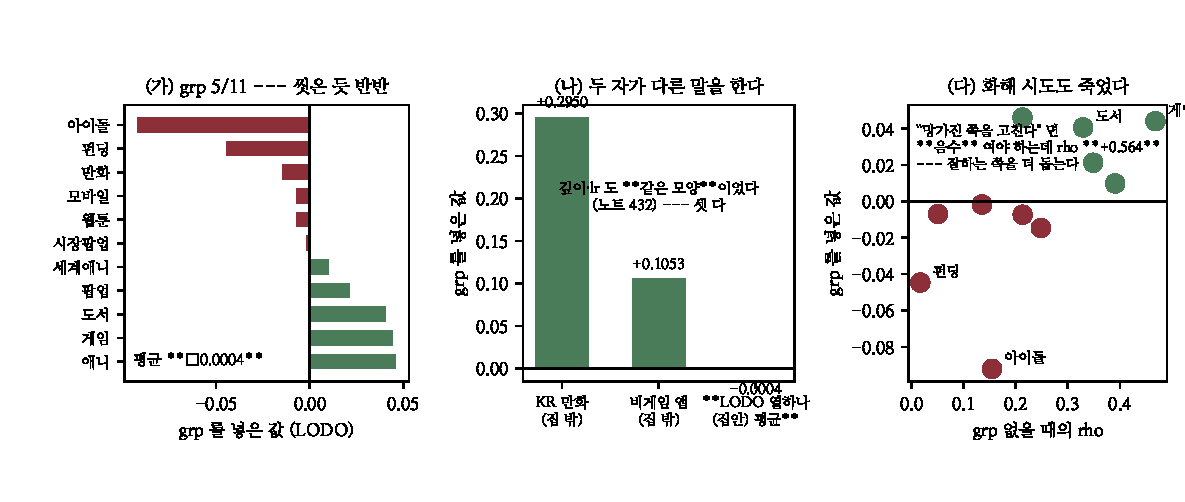
\includegraphics[width=\textwidth]{figs/fig433.pdf}
\caption{(가) LODO 에서 grp 는 반반이다. (나) 두 자가 다른 말을 한다.
(다) ``망가진 쪽을 고친다''는 부호가 반대다.}
\end{figure}

\end{document}
